\subsection{Project}
The wofa-backend\footnote{\url{https://github.com/maurice-herwig/wofa-backend}} project provides endpoints for all the computations provided by the WoFA\footnote{\url{https://github.com/maurice-herwig/wofa}} project to use this project as a microservice in a web architecture. More information about the project and the setup can be found on the GitHub pages. 

\subsection{Authorization}
The WoFa Backend allows only authenticated clients access to this to the services of this backend. To authenticate a client, we must register the new client as an application on the admin site. For this, visit the base\_url/admin site, login with the in the setup step created superuser and add a new application. By adding a new application, we see the following formula fill this with in the fig.~\ref{fig:add_application} seen data and save the client\_id and client\_secret. Important save the values before you save the new application, because after the save the client secret are hashed. 

\begin{figure}
    \centering
    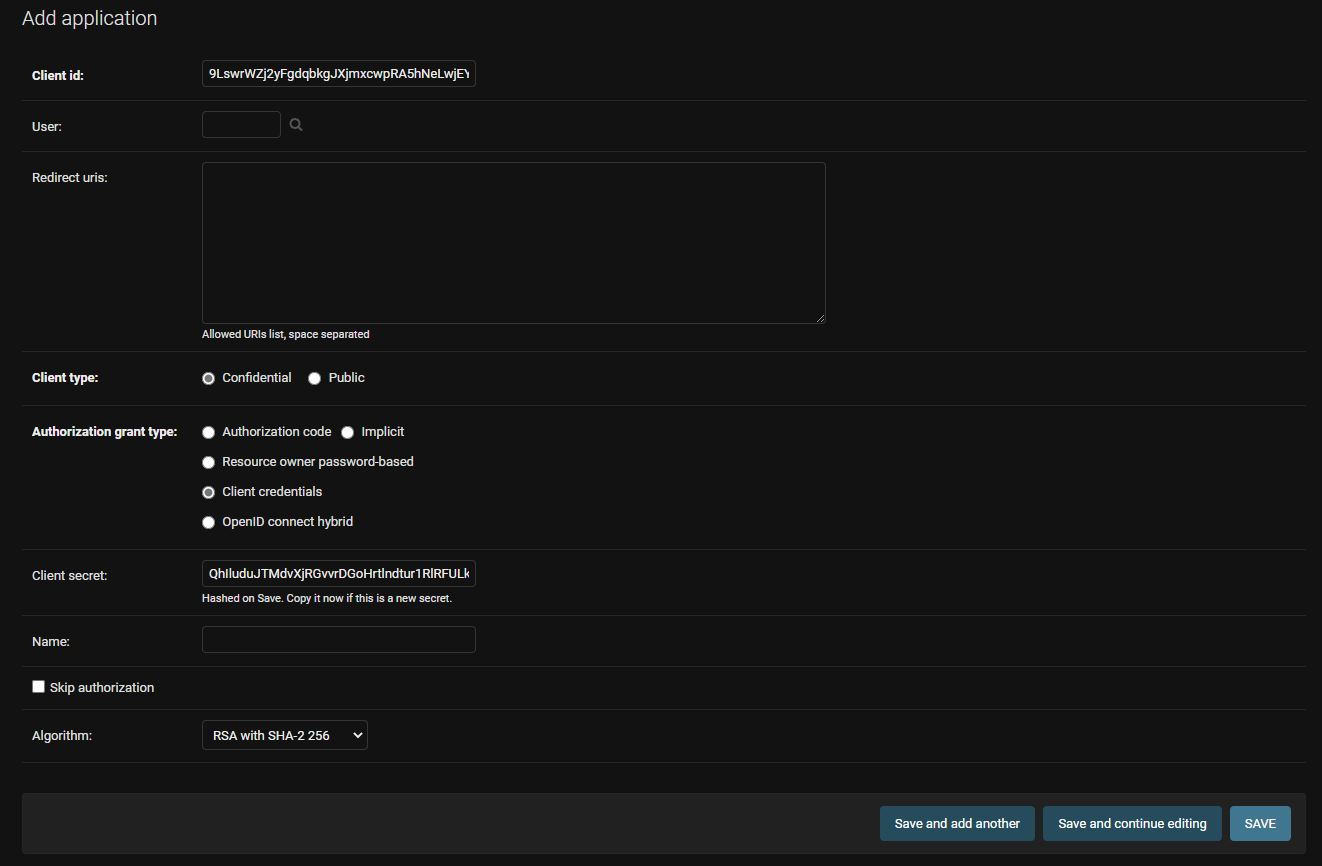
\includegraphics{pictures/register_application.jpg}
    \caption{Formula to add a new application. Choose as client type confidential and as authorization grant type Client credentials. For the encryption, choose RSA. } 
    \label{fig:add_application}
\end{figure}


\subsubsection{POST o/ token/}

\textbf{Description:}\\
\ \\
To get access to all endpoints of this application, we need an access token. That every following request need as a header value. To get this access token, we must send a POST request to the o/token/ endpoint, with the clinet\_id and client\_secret. Important is that the tokens have a limited lifetime, so that we need a new one when the old one expires. The lifetime of a token can we see in the response at the expires\_in field in seconds. \\
\ \\
\textbf{Body:}
\begin{itemize}
    \item client\_id: $\langle$client\_id$\rangle$
    \item client\_secret: $\langle$client\_secret$\rangle$
    \item grant\_type: client\_credentials
\end{itemize}
\ \\
\textbf{Example:} \\
\ \\
\textcolor{blue}{curl -X POST '\BaseURL o/token/'}\\
\textcolor{blue}{-d} \{ 
     \textcolor{red}{"client\_id"}: "PWR2JsaskdvpbcGieDZfNjKfhgw9CW2UoRV6zoH5" 
     \begin{adjustwidth}{7.5 mm}{0 cm}
        \textcolor{red}{"client\_secret"}: e19e3yxbNejQ7bg7ND6vBic4XEVRxXV41oMrEkDqAYGa\dots\\
        \textcolor{red}{"grant\_type"}: "client\_credentials"\}
     \end{adjustwidth}
\ \\
\textbf{Response:}\\
\ \\
\{
\begin{adjustwidth}{7.5 mm}{0 cm}
    \textcolor{red}{"access\_token"}: "sTAovipN0p1mpJ0bRKpQ2ncxD6pUSd",\\
    \textcolor{red}{"expires\_in"}: 3600,\\
    \textcolor{red}{"token\_type"}: "Bearer",\\
    \textcolor{red}{"scope"}: "all"
\end{adjustwidth}
\}
